% !TEX root = ../main.tex
% Einleitung

Das Bedürfnis, Informationen anschaulich darzustellen, ist ein Phänomen, das die Kulturgeschichte des Menschen seit der Frühzeit begleitet. Eine der ältesten visuellen Metaphern ist der Baum.
Dessen grafische Darstellung könnte dabei unterschiedlicher nicht sein, von Abbildungen die nahezu realistisch sind, bis hin zu abstrakten Formen, beispielsweise in Form von einfachen Knoten und Kanten.
Als visuelle Metapher zur Darstellung von Informationen kommen Baumdiagramme in vielen Bereichen zum Einsatz; z.\,B. zur Darstellung von Erbfolgen, der sogenannte Stammbaum, oder um die Rangordnungen im Tierreich abzubilden.
Im Besonderen macht sich diese Darstellungsform folglich die Hierarchie und geordnete Struktur eines Baumes zu Nutzen.
So lässt sich der Baum als eine visuelle Repräsentation verstehen, mit dessen Hilfe sich komplexe Beziehungen zwischen einzelnen Entitäten übersichtlich darstellen lassen.\cite{lima2014book}

Die Arbeit beschäftigt sich einerseits mit der visuellen Metapher des Baums und der darauf aufbauenden Kategorienstruktur von Wikipedia, als auch andererseits mit den Ähnlichkeiten zwischen den einzelnen Paragraphen der in der Wikipedia veröffentlichten Artikeln.
Das Ziel der Arbeit ist es, mittels grafischer Darstellungen und der Möglichkeit der Exploration, das Verständnis über die Datensätze zu verbessern und somit letztlich auch über die Enzyklopädie Wikipedia.

%NOTE
% Relevanz von Informationsvisualisierung\\
% Bezug auf das vorangegangene Projekt Visual Text Analytics\\
% einmal eine Abstrakte Motivation -> Darstellung Kategorienbaum + "Ahnlichkeiten
%
% Motivation aus dem vorg"anger Projekt -> konkreter Bezug auf fehlende Eigenschaften und Erkenntnisse
% defacto die einzige Visualisierung f"ur den Kategoriebaum der Wikipedia
% =========================================================

Die vermeintliche Ordnung der Kategorien innerhalb der Wikipedia von abstrakten und allumfassenden Konzepten auf der höchsten Ebene der Kategorisierung, zu immer spezifischeren Themengebieten, lässt eine stark hierarchische Struktur vermuten.

\section{Motivation}

Im Projekt "`Visual Text Analytics"' wurde bereits ein Versuch unternommen, die Ähnlichkeiten von Wikipedia-Artikeln zu visualisieren.
Der Fokus des Projekts lag auf der Darstellung der inhaltlichen Überschneidungen einer möglichst großen Anzahl von Wikipedia-Artikeln und den Ähnlichkeitswerten zwischen Wikipedia-Artikeln, wie in der Abbildung \ref{fig:vta-cover} gezeigt.
Im Kapitel \ref{subchap:simmatrix}, wird im Detail auf die Berechnung der Ähnlichkeiten eingegangen.
Diese Visualisierung unterstützend werden die zugehörigen Wikipedia-Kategorien in einer separaten Visualisierung als Graph dargestellt.
Dieser die Wikipedia-Katgorien abbildende Graph soll eine verständliche Zusammenfassung auf einer höheren Abstraktionsebene für die Menge der erfassten Wikipedia-Artikel ermöglichen, verdeutlicht in Abbildung \ref{subchap:simmatrix}. 
Dabei werden die Wikipedia-Artikel aus Abbildung \ref{fig:vta-cover}, anhand eines im voraus festgelegten Schwellwerts nach Ähnlichkeiten in Clustern gebündelt.
Die Bestimmung eines initialen Schwellwerts vor der Visualisierung legt dabei fest, bis zu welchem Ähnlichkeitswert Artikel zu Clustern gebündelt werden. Ähnlichkeitswerte unter dem Schwellwert werden nicht mehr in Betracht gezogen. 
Die Änderung des Schwellwerts während der Visualisierung, um Ähnlichkeitswerte in Form von Kanten hinzuzufügen, ist nicht ohne eine Überlappung von Kanten möglich.
Durch die massive Überzeichnen von Elementen ist es nur schwer möglich, aus der Visualisierung etwas zu verstehen. Die damit einhergehende eingeschränkte Interaktivität mit den Daten ist das Grundproblem dieses Projektes.


%Diese Vorgehensweise erschwert jedoch eine dynamische Darstellung, da die Bestimmung eines Schwellwerts die Anordnung der Knoten und Kanten festlegt, weshalb der Schwellwert für die Dauer des Programms statisch bleibt.
%Es besteht die Möglichkeit den Schwellwert zu ändern, doch dadurch würden die neu gezeichneten Kanten so angeordnet, dass eine Vielzahl an Überlappungen entstünden.

% \paragraph{Ziel}
Den Impuls zur vorliegenden Arbeit gaben die Beobachtungen aus diesem Projekt \emph{Visual Text Analytics}.
Im Laufe der Projektarbeit wurden Schwachstellen identifiziert und Mängel herausgestellt, die im Rahmen dieser Untersuchung weiterbearbeitet wurden.
Der Fokus dieser Forschungsarbeit liegt dabei auf der Entwicklung einer geeigneten Darstellung von Verbindungen zwischen den Kategorien der Wikipedia.
Eine Anforderung, die an eine Visualisierung von Informationen gestellt wird, ist, Knoten und Kanten zu finden, bei denen die Überlappung möglichst gering ist. Zugleich soll auch eine mögliche Anpassung des Schwellwerts gewährleistet werden, dass die Überlappungen der dargestellten Elemente weiterhin möglichst niedrig bleibt.
Die Suche nach den Kategorien und die interaktive Exploration der Verbindungen zwischen den Kategorien steht dabei im Mittelpunkt.
Des Weiteren setzt sich die Arbeit mit der Entwicklung einer Strategie auseinander, um eine dünn besetzte Matrix in der Größe von 643 GB zu veranschaulichen und zugänglich zu machen.
Die Arbeit zielt darauf ab, das Verständnis über die Enzyklopädie Wikipedia zu schärfen und zu vertiefen.


\begin{figure}
\centering
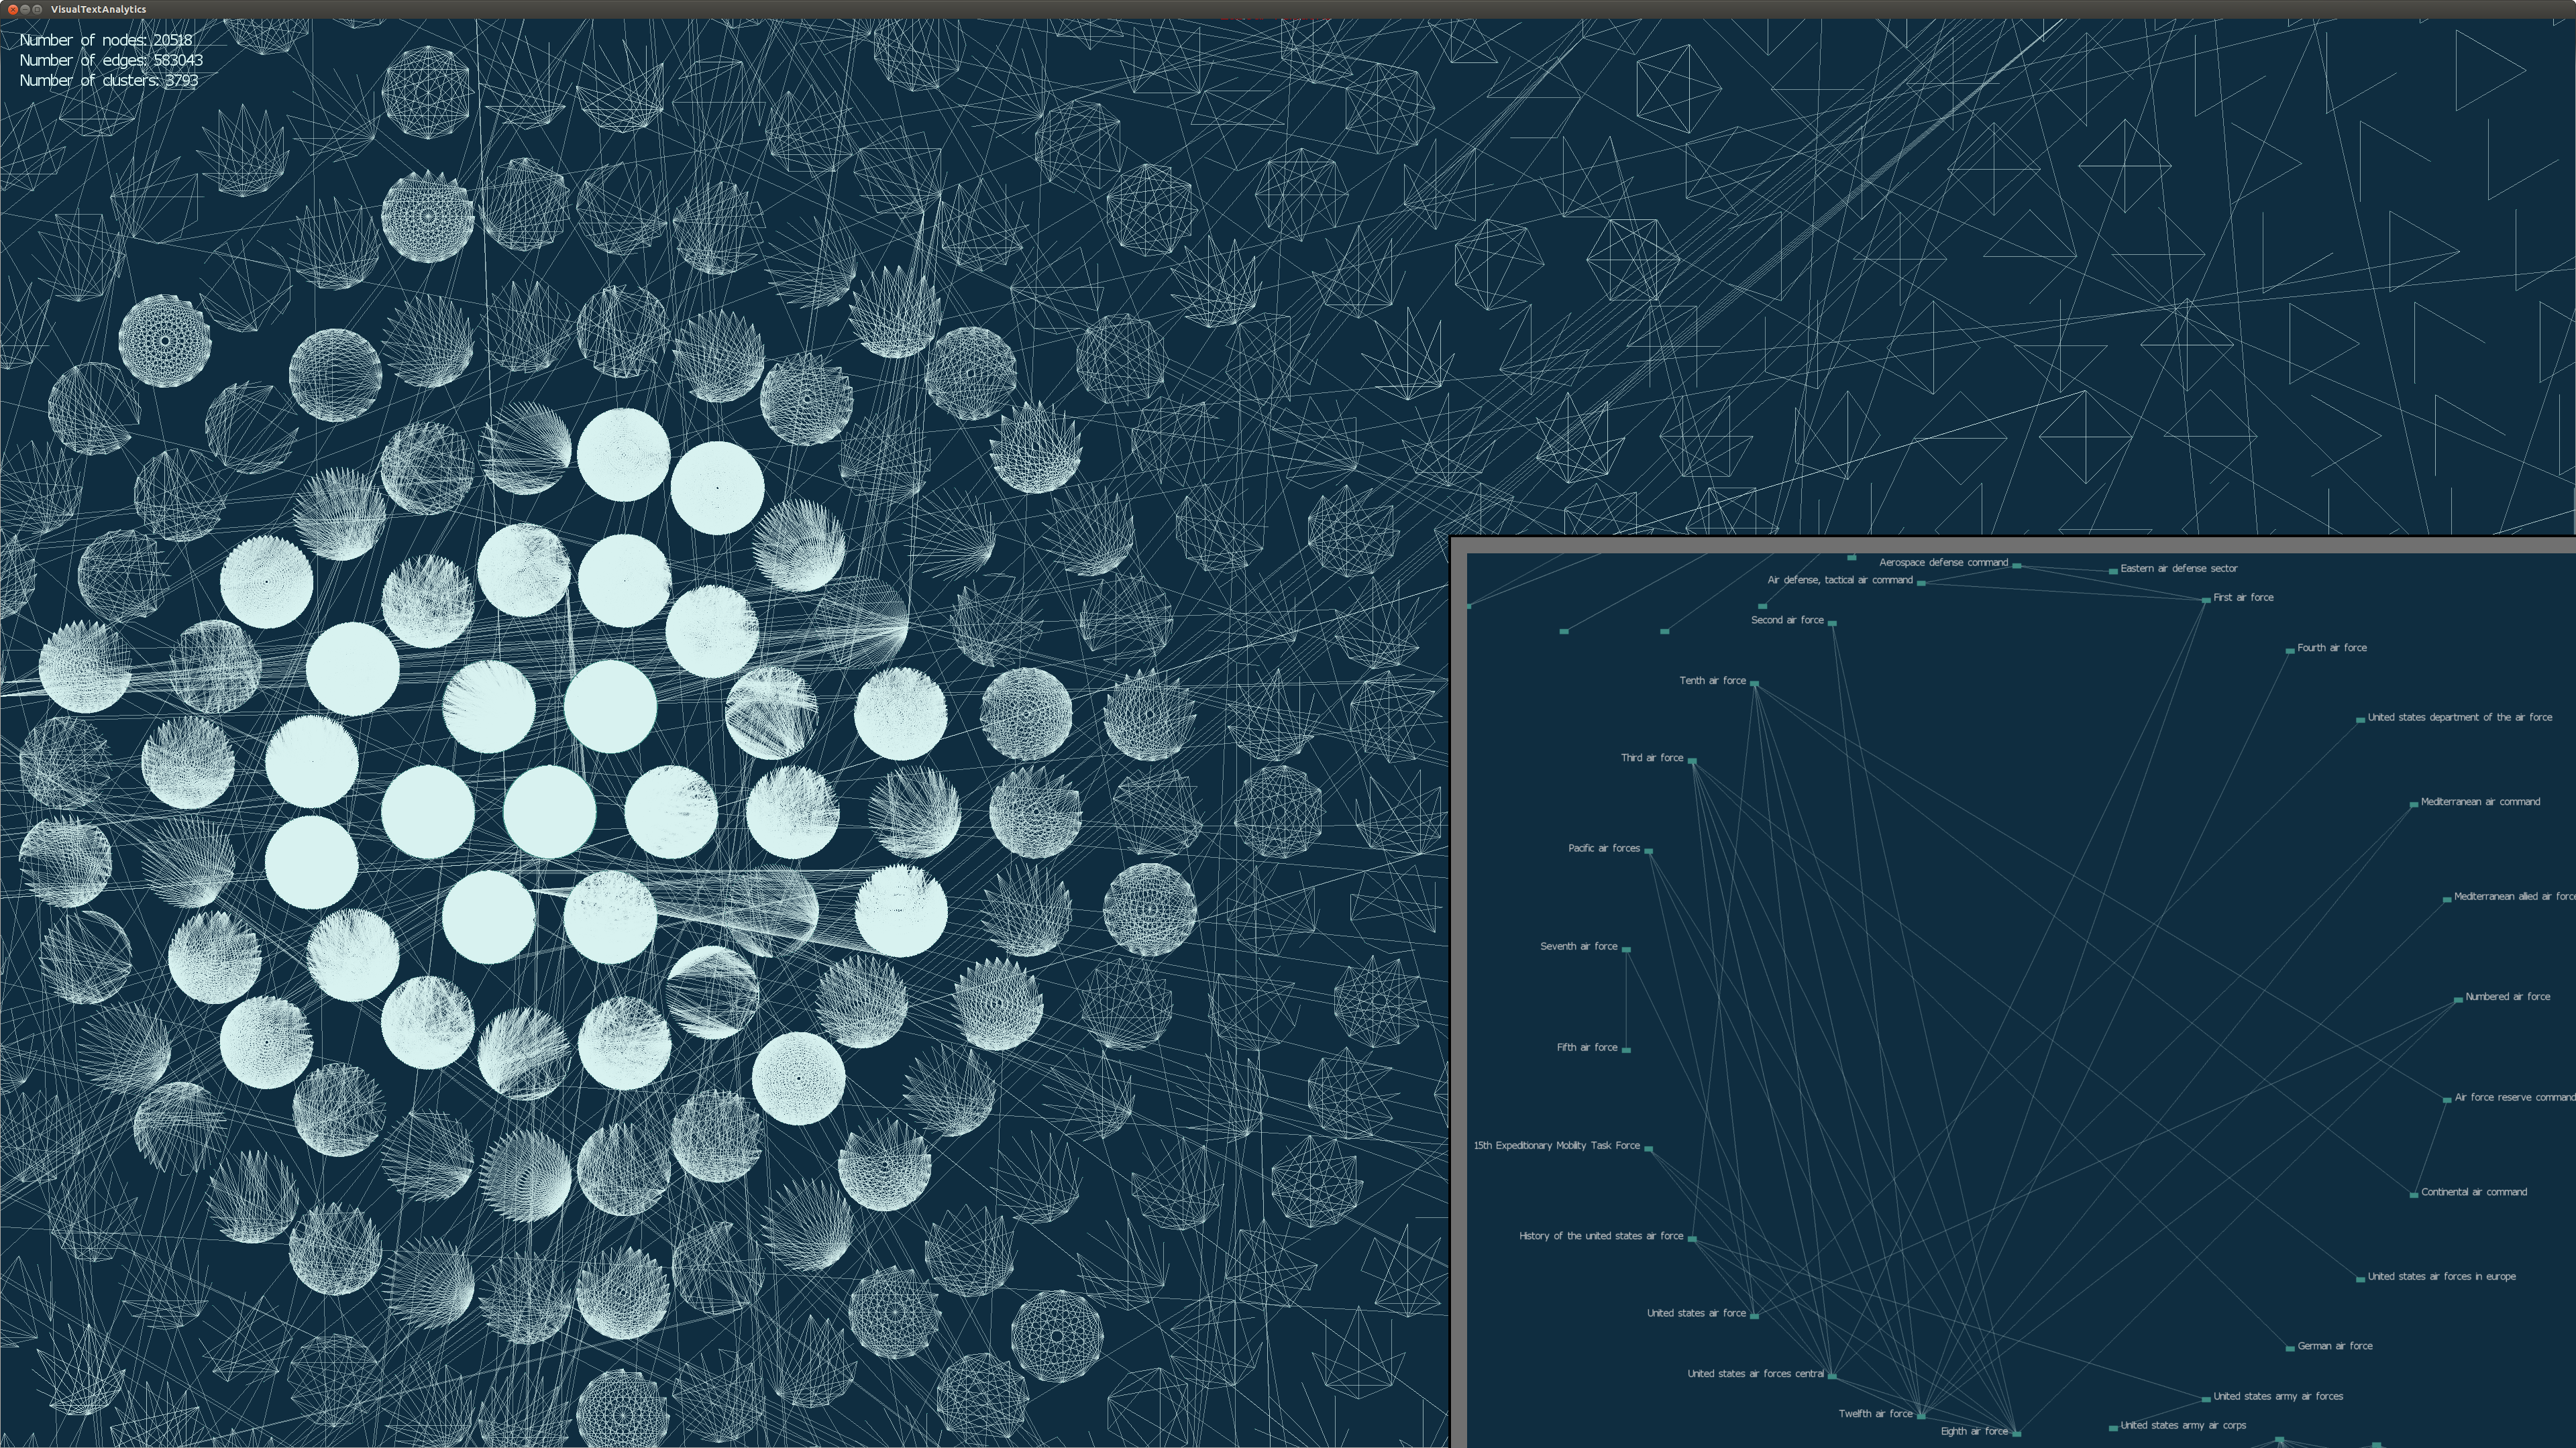
\includegraphics[width=\textwidth]{images/01_introduction/vta-cover.png}
\caption{Ausschnitt aus dem Projekt \textit{Visual Text Analtytics}. Rechts unten ist ein Cluster im Fokus zu sehen. Der Hintergrund zeigt die Startvisualisierung mit einer Übersicht aller Cluster.}
\label{fig:vta-cover}
\end{figure}

\begin{figure}
    \centering
    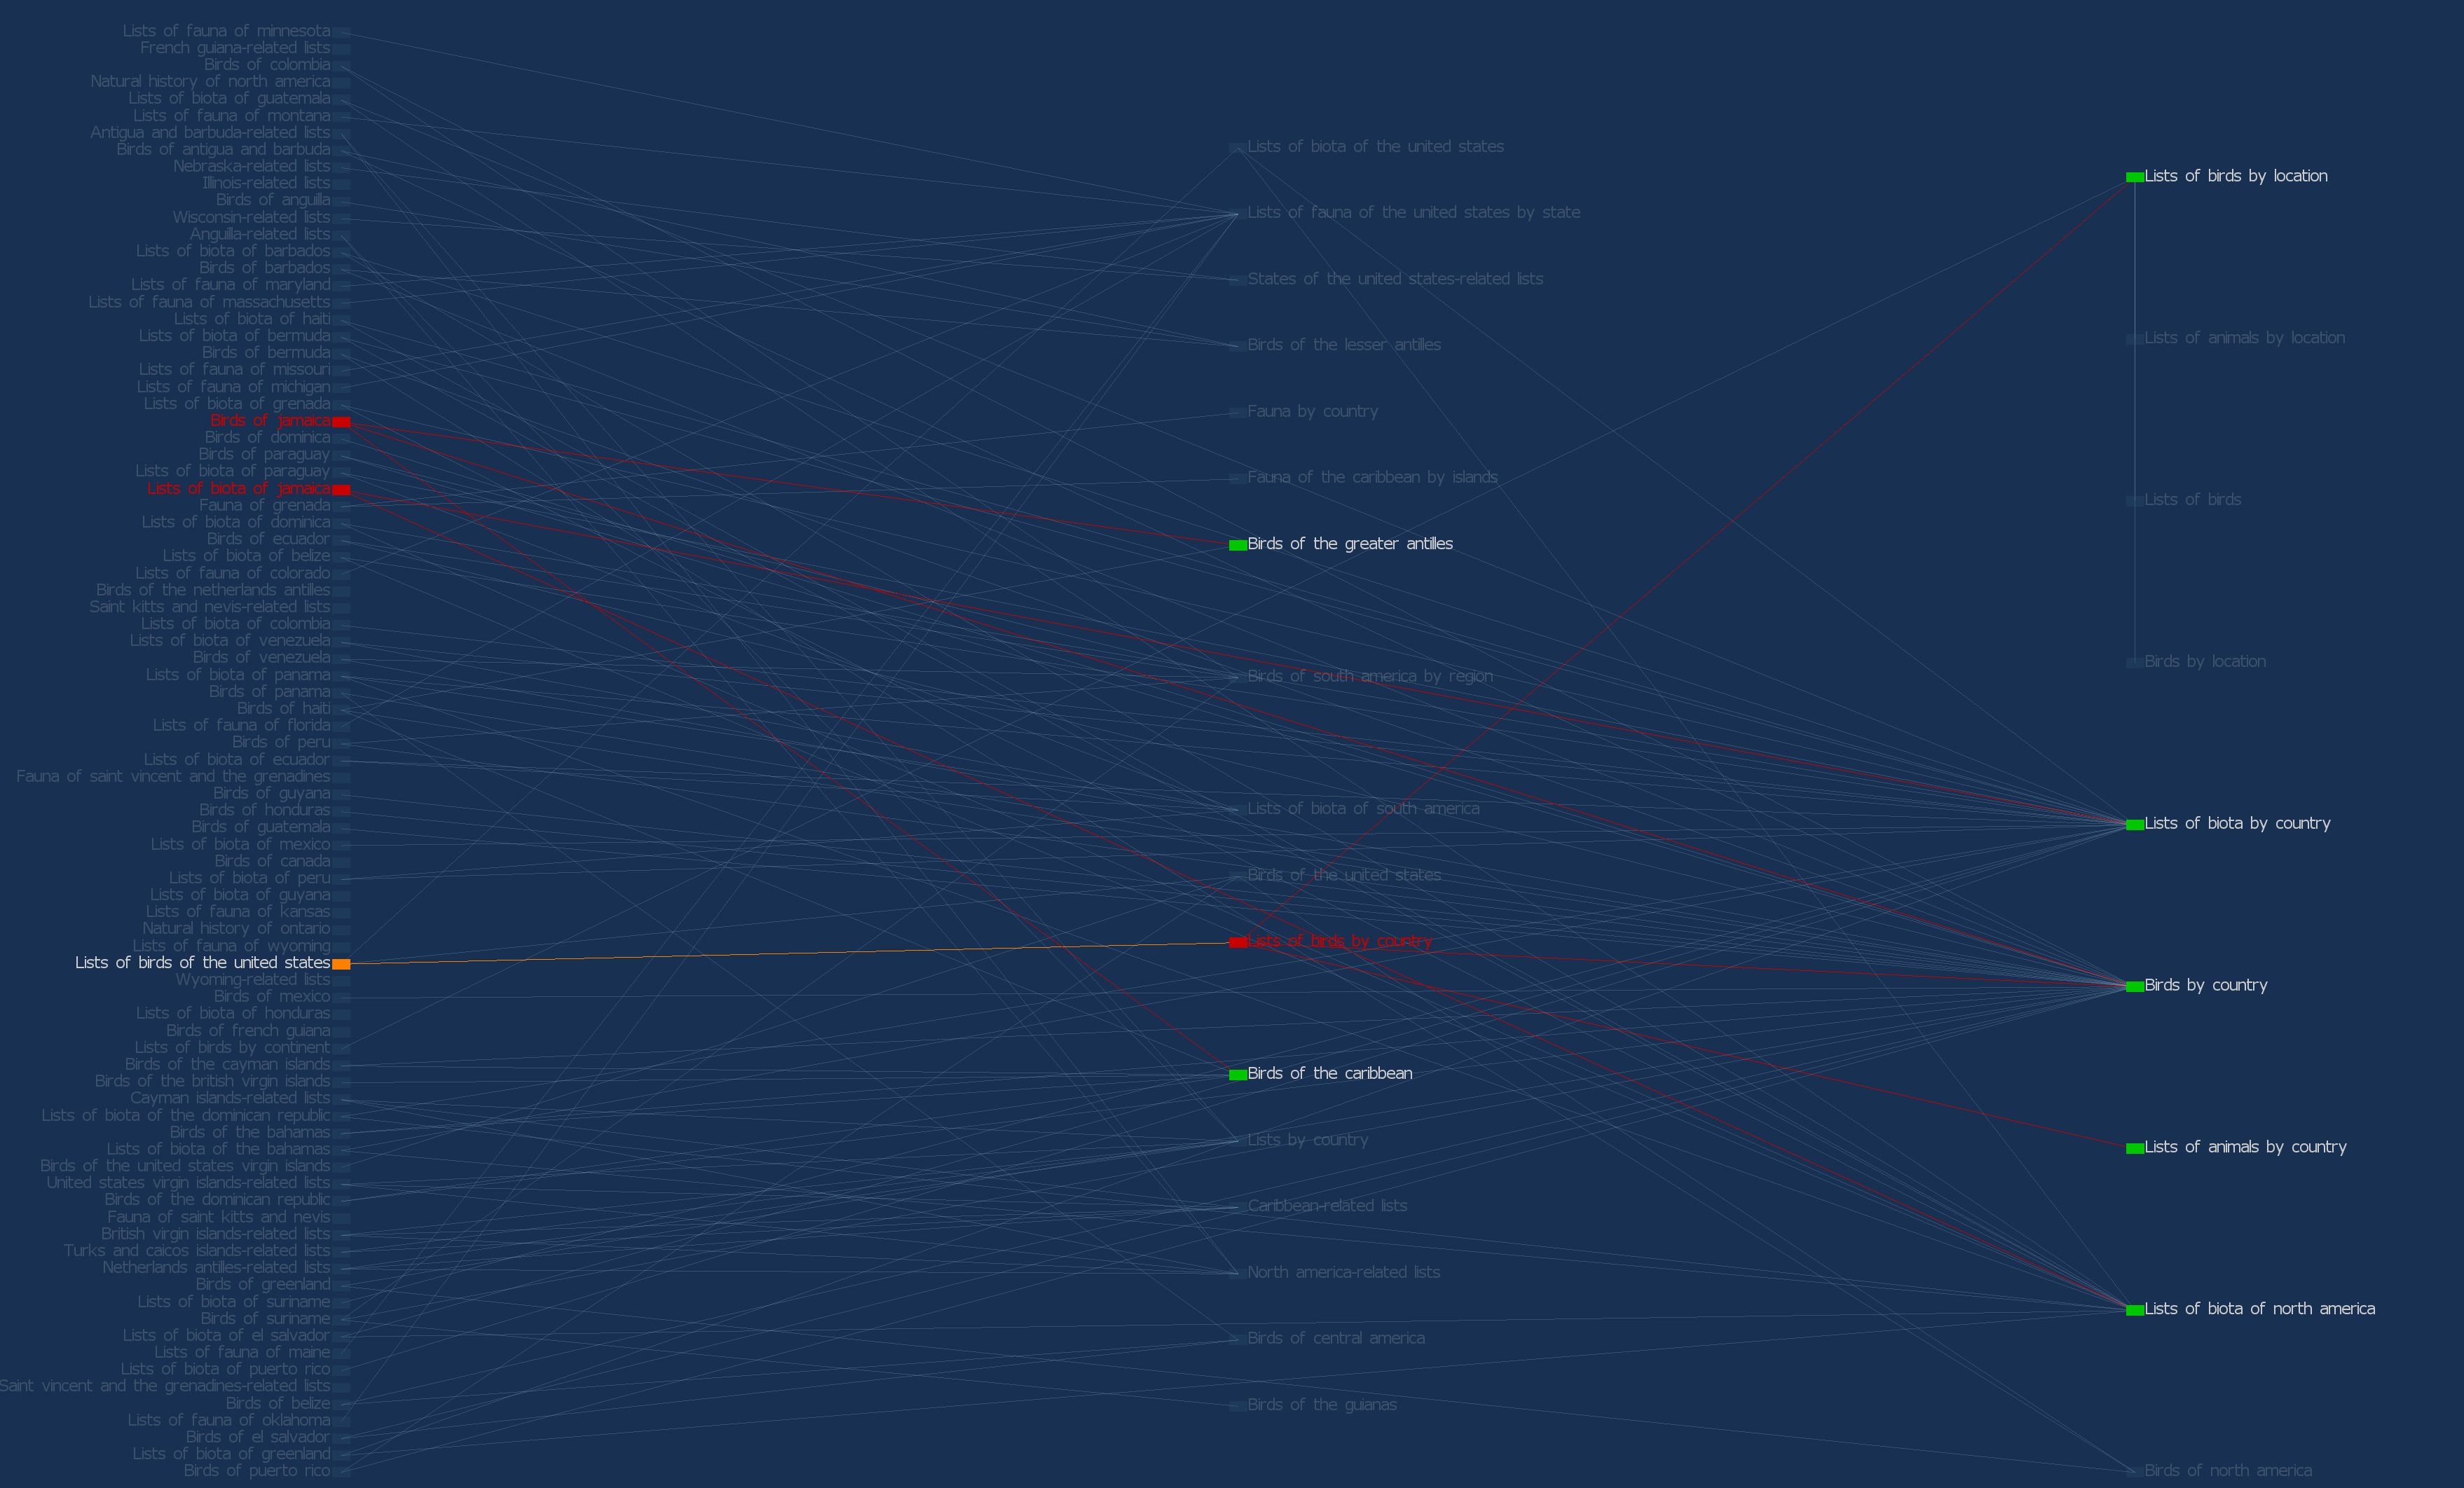
\includegraphics[width=\textwidth]{images/01_introduction/category-view.png}
    \caption{Ausschnitt des Kategoriengraphen. Die Knoten stellen Kategorien dar und die Kanten veranschaulichen die Verbindungen zwischen den Kategorien.\\ In diesem Bild wird die grün gefärbte Kategorie ausgewählt. Alle Knoten und Kanten ohne Verbindung zur ausgewählten Kategorie sind ausgegraut.}
    \label{fig:category-view}
\end{figure}
\todotext{bild mit einer geclickten Kategorie}










% DRAFTS ============================
% Um die enorme Menge an Kanten, welche einen Vergleich zwischen zwei Artikeln repres"antiert, darstellen zu k"onnen, muss ein Schwellwert festgelegt werden, bevor die Visualisierng ausgef"uhrt wird.

% Ziel der Arbeit ist es, das Verst"andnis "uber die Kategoriestruktur und die "Ahnlichkeiten zwischen Artikeln der Wikipedia zu verbessern.
% F"ur die enorme Menge an Vergleichen zwischen Artikeln muss eine L"osung entwickelt werden, welche die Menge reduziert, somit f"ur den Computer darstellbar und f"ur den Menschen nachvollziehbar ist.
% Der Mittelpunkt der Arbeit ist die Darstellung der hierarchischen Struktur der Kategorien aus der Wikipedia.

% BULLET LIST ++++++++++++++++++++++++++++++++++++++++++++++++
% \begin{itemize}
%   \item Bedeutung des Wikipediadatensatzes
%   \item Kritikpunkte im Projekt Visual Text Analytics
%   \begin{itemize}
%     \item statisches Layout
%     \item fehlende M"oglichkeit zur Exploration der Daten
%     \item "Ubersicht der Visualisierung ist sehr undurchsichtig
%     \item Schwierigkeiten beim Nachvollziehen der Verbindungen zwischen den Artikeln untereinander
%     \item "Anderung des Schwellwertes f"ur "Ahnlichkeiten -> zu viele Kanten
%     \item fehlende M"oglichkeit, die Auswahl an Artikeln einzuschr"anken
%     \item Unterst"utzende Funktion zum Zusammenfassen von mehreren Artikeln -> Kategorien, Cluster
%     \item Artikelcluster mit vielen "Ahnlichkeiten zueinander sind schwer zu lesen
%     \item Kategorienbaum unzureichend als Unterzt"utzung neben den Artikeln
%   \end{itemize}
% \end{itemize}


% \begin{itemize}
%     \item Verbesserung des Verst"andnisses des "Ahnlichkeitsma"ses
%     \item Darstellung der Hierarchie von Kategorien
%     \begin{itemize}
%       \item Konstruktion eines Kategorienbaumes mit der M"oglichkeit der Exploration
%     \end{itemize}
%     \item Interaktive Visualisierung
%     \begin{itemize}
%       \item "Anderung des Schwellwerts zur Laufzeit
%     \end{itemize}
%     \item Exploration der Daten
%     \item Bezug zu anderen Datens"atzen: Autoren, Editierungen, etc.
% \end{itemize}














































% % ////////////////////////////////////
% \begin{figure}[H]
%     \centering
%     \begin{subfigure}[b]{0.96\textwidth}
%         \includegraphics[width=\textwidth]{images/01_introduction/motivation_temporal_superresolution_one.pdf}
%         \caption{3D video playback rate matching the low recording rate}
%         % \label{subfig:playback_rate_matching}
%     \end{subfigure}

% 	\vspace{1.0cm}

%     \begin{subfigure}[b]{0.96\textwidth}
%         \includegraphics[width=\textwidth]{images/01_introduction/motivation_temporal_superresolution_two.pdf}
%         \caption{3D video playback matching the video encoding standards to ensure persistence of fluid motion}
%         % \label{subfig:playback_rate_higher}
%     \end{subfigure}
%     \caption[Concept of Temporal Super Resolution in a 3D Video Player]{In this Figure, two different playback rates for a low frame rate recording of a 3D volume sequence is presented. The tick marks on the black arrows indicate the position of recorded frames. The blue arrows indicate the playback rate that matches the recording \subref{subfig:playback_rate_matching} and an increased playback rate \subref{subfig:playback_rate_higher} using temporal interpolation to provide the viewer with a impression of fluid motion. }
%     % \label{fig:temporal_superresolution}
% \end{figure}

%  \cite{VillanuevaEtAl:2016}